% ============================================================================
%  Exam Question Difficulty Predictor — Technical Report
%  Intelligent Question Complexity Analysis via Feature Engineering & XGBoost
% ============================================================================
\documentclass[12pt, a4paper]{article}

% --- Packages ---------------------------------------------------------------
\usepackage[utf8]{inputenc}
\usepackage[T1]{fontenc}
\usepackage{lmodern}
\usepackage[margin=1in]{geometry}
\usepackage{graphicx}
\usepackage{booktabs}
\usepackage{array}
\usepackage{amsmath, amssymb}
\usepackage{xcolor}
\usepackage{hyperref}
\usepackage{enumitem}
\usepackage{caption}
\usepackage{subcaption}
\usepackage{float}
\usepackage{listings}
\usepackage{fancyhdr}
\usepackage{titlesec}
\usepackage{tocloft}
\usepackage{parskip}
\usepackage{multirow}
\usepackage{tabularx}
\usepackage{longtable}
\usepackage{tikz}
\usetikzlibrary{shapes.geometric, arrows.meta, positioning, calc, fit, backgrounds}

% --- Colour Palette (Slate-700 / Slate-400 / Blue-600) ----------------------
\definecolor{primary}{HTML}{334155}
\definecolor{accent}{HTML}{2563EB}
\definecolor{muted}{HTML}{94A3B8}
\definecolor{codebg}{HTML}{F1F5F9}
\definecolor{linkblue}{HTML}{3B82F6}

% --- Hyperref Setup ---------------------------------------------------------
\hypersetup{
    colorlinks  = true,
    linkcolor   = primary,
    urlcolor    = linkblue,
    citecolor   = accent,
    pdftitle    = {Exam Question Difficulty Predictor — Technical Report},
    pdfauthor   = {Rishik Chowdary Karuturi},
}

% --- Header / Footer --------------------------------------------------------
\pagestyle{fancy}
\fancyhf{}
\fancyhead[L]{\small\textcolor{muted}{Exam Question Difficulty Predictor}}
\fancyhead[R]{\small\textcolor{muted}{Technical Report}}
\fancyfoot[C]{\thepage}
\renewcommand{\headrulewidth}{0.4pt}

% --- Section Styling --------------------------------------------------------
\titleformat{\section}
  {\Large\bfseries\color{primary}}{\thesection}{1em}{}[\vspace{-0.5em}\textcolor{muted}{\rule{\textwidth}{0.4pt}}]
\titleformat{\subsection}
  {\large\bfseries\color{primary}}{\thesubsection}{1em}{}
\titleformat{\subsubsection}
  {\normalsize\bfseries\color{primary}}{\thesubsubsection}{1em}{}

% --- Code Listing Style -----------------------------------------------------
\lstdefinestyle{pythonstyle}{
    backgroundcolor=\color{codebg},
    basicstyle=\ttfamily\small,
    keywordstyle=\color{accent}\bfseries,
    commentstyle=\color{muted}\itshape,
    stringstyle=\color{primary},
    breaklines=true,
    frame=single,
    rulecolor=\color{muted},
    numbers=left,
    numberstyle=\tiny\color{muted},
    xleftmargin=2em,
    framexleftmargin=1.5em,
}
\lstset{style=pythonstyle}

% ============================================================================
%  DOCUMENT BEGIN
% ============================================================================
\begin{document}

% --- Title Page -------------------------------------------------------------
\begin{titlepage}
\begin{center}
    \vspace*{2cm}

    {\Huge\bfseries\textcolor{primary}{Exam Question Difficulty Predictor}}\\[0.6cm]
    {\Large\textcolor{muted}{Intelligent Question Complexity Analysis\\via Feature Engineering \& XGBoost}}

    \vspace{1.5cm}

    \textcolor{muted}{\rule{0.6\textwidth}{0.4pt}}

    \vspace{1.5cm}

    {\large
    \textbf{Authors:}\\[0.3cm]
    Rishik Chowdary Karuturi\\[0.15cm]
    Palwai Tejaswini\\[0.15cm]
    Nakkina Lakshmi Praneeth\\[0.5cm]
    \textbf{Date:} February 2026\\[0.3cm]
    \textbf{Version:} 1.0
    }

    \vspace{2cm}

    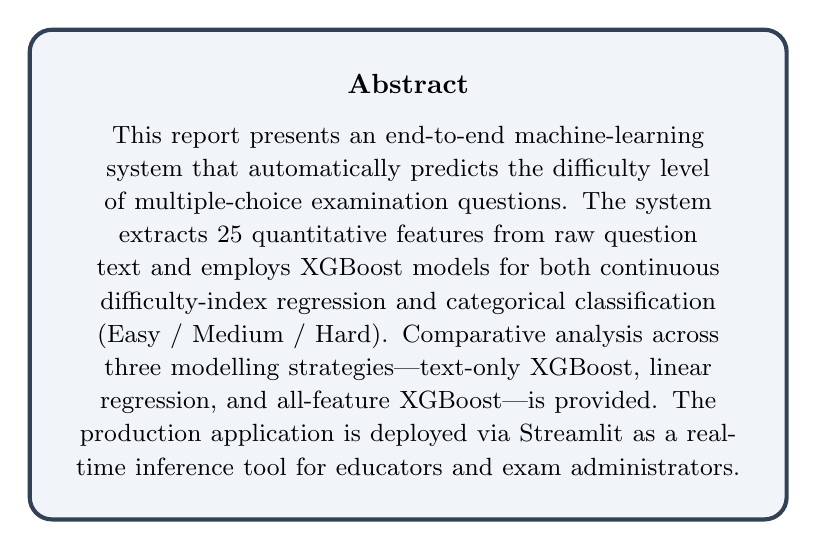
\begin{tikzpicture}
        \node[draw=primary, rounded corners=8pt, line width=1.5pt,
              inner sep=16pt, text width=0.7\textwidth, align=center,
              fill=codebg] {
            \textbf{Abstract}\\[6pt]
            \small
            This report presents an end-to-end machine-learning system that
            automatically predicts the difficulty level of multiple-choice
            examination questions. The system extracts 25~quantitative features
            from raw question text
            and employs XGBoost models for both continuous difficulty-index
            regression and categorical classification (Easy / Medium / Hard).
            Comparative analysis across three modelling strategies—text-only
            XGBoost, linear regression, and all-feature XGBoost—is provided.
            The production application is deployed via Streamlit as a real-time
            inference tool for educators and exam administrators.
        };
    \end{tikzpicture}

    \vfill
    {\small\textcolor{muted}{GenAI Project — Machine Learning Pipeline \& Streamlit Application}}
\end{center}
\end{titlepage}

% --- Table of Contents ------------------------------------------------------
\tableofcontents
\newpage

% ============================================================================
%  1. INTRODUCTION
% ============================================================================
\section{Introduction}\label{sec:intro}

\subsection{Motivation}
Educators, instructional designers, and testing organisations invest considerable manual effort in evaluating the difficulty and quality of examination questions. A misjudged question can skew test results and inaccurately measure student proficiency. Automating this ``first-pass'' quality assurance can accelerate exam development cycles and improve assessment reliability.

\subsection{Objective}
The \textbf{Exam Question Difficulty Predictor} is an end-to-end, production-structured machine-learning pipeline that:
\begin{enumerate}[leftmargin=2em]
    \item Takes raw question text—including \LaTeX\ and mathematical symbols—as input.
    \item Extracts \textbf{25 quantitative features} spanning lexical, mathematical, and domain-specific dimensions.
    \item Predicts a continuous \textbf{difficulty index} ($p$-value, $0.0$–$1.0$) via regression.
    \item Classifies the question into a categorical \textbf{difficulty tier}: Easy, Medium, or Hard.
    \item Exposes predictions through an interactive \textbf{Streamlit web application}.
\end{enumerate}

\subsection{Scope}
\begin{itemize}[leftmargin=2em]
    \item \textbf{Domain:} English-language mathematics examination questions.
    \item \textbf{Dataset:} 50{,}000 preprocessed exam questions with associated metadata.
    \item \textbf{Models:} XGBoost (primary), Linear Regression (baseline).
    \item \textbf{Deployment:} Local Streamlit application with serialised model artefacts.
\end{itemize}

% ============================================================================
%  2. DATASET
% ============================================================================
\section{Dataset}\label{sec:dataset}

\subsection{Source \& Scale}
The dataset comprises \textbf{50{,}000 examination questions} sourced from educational repositories. Each record contains:
\begin{itemize}[leftmargin=2em]
    \item Question text (may include \LaTeX)
    \item Four multiple-choice answer options (A–D)
    \item Continuous difficulty $p$-value ($0.0 =$ hardest, $1.0 =$ easiest)
    \item Categorical difficulty label (Easy / Medium / Hard)
    \item Subject metadata, misconception counts, and construct frequency
    \item Post-administration statistics (response time, discrimination index, IRT parameters)
\end{itemize}

\subsection{Data Cleaning Pipeline}
A dedicated preprocessing script (\texttt{clean\_dataset.py}) applies the following transformations:

\begin{center}
\renewcommand{\arraystretch}{1.3}
\begin{tabularx}{\textwidth}{>{\bfseries}l X}
    \toprule
    Step & Description \\
    \midrule
    NULL Standardisation & Unifies heterogeneous null markers (\texttt{N/A}, \texttt{none}, \texttt{?}, \texttt{--}) into \texttt{NaN}. \\
    Whitespace Stripping & Removes leading/trailing whitespace from all string columns. \\
    Deduplication        & Identifies and removes identical rows. \\
    Casing Normalisation & Standardises categorical fields to title case. \\
    Domain Constraints   & Enforces $p$-value and percentage fields into $[0, 1]$ or $[0, 100]$. \\
    Outlier Capping      & Applies inter-quartile range (IQR) capping to numeric distributions. \\
    Type Coercion        & Forces correct \texttt{dtypes} (float, int, category). \\
    \bottomrule
\end{tabularx}
\end{center}

\subsection{Class Distribution}
The dataset exhibits significant class imbalance:

\begin{center}
\renewcommand{\arraystretch}{1.3}
\begin{tabular}{lrr}
    \toprule
    \textbf{Class} & \textbf{Approx.\ Count} & \textbf{Proportion} \\
    \midrule
    Easy   & $\sim$40{,}000 & $\sim$80\% \\
    Medium & $\sim$7{,}500  & $\sim$15\% \\
    Hard   & $\sim$2{,}500  & $\sim$5\%  \\
    \bottomrule
\end{tabular}
\end{center}

\noindent This imbalance is a critical consideration discussed in Section~\ref{sec:results}.

% ============================================================================
%  3. FEATURE ENGINEERING
% ============================================================================
\section{Feature Engineering}\label{sec:features}

All features are extracted by the \texttt{feature\_extractor.py} module. The 25 features fall into six categories:

\subsection{Lexical Features (4)}
\begin{center}
\renewcommand{\arraystretch}{1.2}
\begin{tabular}{ll}
    \toprule
    \textbf{Feature} & \textbf{Description} \\
    \midrule
    \texttt{text\_length}     & Total character count of the question. \\
    \texttt{word\_count}      & Total word count. \\
    \texttt{sentence\_count}  & Sentence count (split on \texttt{.!?}). \\
    \texttt{avg\_word\_length} & Mean number of characters per word. \\
    \bottomrule
\end{tabular}
\end{center}

\subsection{\LaTeX\ \& Mathematical Features (5)}
\begin{center}
\renewcommand{\arraystretch}{1.2}
\begin{tabular}{ll}
    \toprule
    \textbf{Feature} & \textbf{Description} \\
    \midrule
    \texttt{latex\_command\_count}  & Count of detected \LaTeX\ commands. \\
    \texttt{has\_latex}             & Binary indicator ($0/1$). \\
    \texttt{latex\_density}         & $\frac{\texttt{latex\_command\_count}}{\texttt{word\_count}}$. \\
    \texttt{math\_operator\_count}  & Count of operators ($+, -, \times, \div, =$, etc.). \\
    \texttt{number\_count}          & Count of numeric literals. \\
    \bottomrule
\end{tabular}
\end{center}

\subsection{Vocabulary \& Complexity (2)}
\begin{center}
\renewcommand{\arraystretch}{1.2}
\begin{tabular}{ll}
    \toprule
    \textbf{Feature} & \textbf{Description} \\
    \midrule
    \texttt{vocab\_richness}          & $\frac{|\text{unique words}|}{|\text{total words}|}$. \\
    \texttt{text\_complexity\_score}   & Weighted composite: $0.3 \cdot \overline{w} + 0.2 \cdot L + 0.15 \cdot M + 0.1 \cdot N + 2.0 \cdot \frac{L+M}{W}$. \\
    \bottomrule
\end{tabular}
\end{center}

\noindent Where $\overline{w}$ = avg word length, $L$ = \LaTeX\ count, $M$ = math ops, $N$ = numbers, $W$ = word count.

\subsection{Answer-Option Features (5)}
\begin{center}
\renewcommand{\arraystretch}{1.2}
\begin{tabular}{ll}
    \toprule
    \textbf{Feature} & \textbf{Description} \\
    \midrule
    \texttt{answer\_\{a,b,c,d\}\_length}    & Character length of each option. \\
    \texttt{avg\_answer\_length}              & Mean across four options. \\
    \texttt{answer\_length\_variance}         & Variance across four options. \\
    \bottomrule
\end{tabular}
\end{center}

\subsection{Domain-Detection Features (4)}
Binary indicators set to 1 when any keyword from the corresponding dictionary is detected:

\begin{center}
\renewcommand{\arraystretch}{1.2}
\begin{tabular}{lp{8cm}}
    \toprule
    \textbf{Feature} & \textbf{Keyword Examples} \\
    \midrule
    \texttt{has\_advanced\_terms}  & calculus, derivative, integral, eigenvalue, matrix \\
    \texttt{has\_algebra\_terms}   & equation, polynomial, quadratic, factorise, inequality \\
    \texttt{has\_geometry\_terms}  & angle, triangle, circle, hypotenuse, Pythagoras \\
    \texttt{has\_stats\_terms}     & mean, median, probability, histogram, standard deviation \\
    \bottomrule
\end{tabular}
\end{center}

\subsection{Metadata Features (5)}
\begin{center}
\renewcommand{\arraystretch}{1.2}
\begin{tabular}{ll}
    \toprule
    \textbf{Feature} & \textbf{Description} \\
    \midrule
    \texttt{num\_misconceptions}         & Count of associated student misconceptions. \\
    \texttt{has\_misconception}           & Binary ($0/1$). \\
    \texttt{subject\_difficulty\_tier}    & Ordinal tier (1–5) provided by the user. \\
    \texttt{construct\_frequency}         & Frequency of the tested construct in the syllabus. \\
    \bottomrule
\end{tabular}
\end{center}

\noindent\textbf{Crucially,} all 25 \texttt{TEXT\_FEATURES} are available \emph{before} the exam is administered, avoiding data leakage.

% ============================================================================
%  4. MODEL ARCHITECTURE
% ============================================================================
\section{Model Architecture}\label{sec:models}

Three modelling strategies were explored:

\subsection{Model A — XGBoost (Text-Only Features)}
An XGBoost ensemble trained exclusively on the 25 text-derived features. Two sub-models are trained:

\begin{itemize}[leftmargin=2em]
    \item \textbf{Regressor} (\texttt{xgb.XGBRegressor}): Predicts the continuous $p$-value.
    \item \textbf{Classifier} (\texttt{xgb.XGBClassifier}): Predicts the categorical label.
\end{itemize}

\noindent Hyperparameters:

\begin{center}
\renewcommand{\arraystretch}{1.2}
\begin{tabular}{ll}
    \toprule
    \textbf{Parameter} & \textbf{Value} \\
    \midrule
    \texttt{n\_estimators}    & 500 \\
    \texttt{max\_depth}       & 6 \\
    \texttt{learning\_rate}   & 0.05 \\
    \texttt{subsample}        & 0.8 \\
    \texttt{colsample\_bytree} & 0.8 \\
    \texttt{objective (clf)}  & \texttt{multi:softprob} \\
    \texttt{eval\_metric (clf)} & \texttt{mlogloss} \\
    \texttt{objective (reg)}  & \texttt{reg:squarederror} \\
    \bottomrule
\end{tabular}
\end{center}

\subsection{Model B — Linear Regression (Text-Only Features)}
A standard \texttt{sklearn.linear\_model.LinearRegression} trained on the same 25 features as a baseline comparator. No classification model is produced.

\subsection{Model C — XGBoost (All Features)}
An XGBoost ensemble trained on all available features, including \textbf{post-administration} statistics:
\begin{itemize}[leftmargin=2em]
    \item All 25 text features from Model~A
    \item Average response time, response time standard deviation
    \item Discrimination index
    \item IRT difficulty, IRT discrimination, IRT guessing parameters
    \item Student attempt statistics
\end{itemize}

\noindent\textbf{Important:} Post-admin features are only available \emph{after} an exam has been administered. This model demonstrates the upper-bound performance but entails target leakage for cold-start deployment.

% ============================================================================
%  5. TRAINING & EVALUATION
% ============================================================================
\section{Training \& Evaluation}\label{sec:training}

\subsection{Data Split}
\begin{itemize}[leftmargin=2em]
    \item \textbf{Train:} 80\% of the dataset
    \item \textbf{Test:} 20\% of the dataset
    \item Stratified split on \texttt{difficulty\_label} to preserve class proportions.
\end{itemize}

\subsection{Cross-Validation}
5-fold stratified cross-validation is applied to the classification models using \texttt{sklearn.model\_selection.cross\_val\_score} with accuracy scoring.

\subsection{Evaluation Metrics}

\subsubsection{Regression}
\begin{itemize}[leftmargin=2em]
    \item \textbf{MAE} (Mean Absolute Error): $\frac{1}{n}\sum_{i=1}^{n}|y_i - \hat{y}_i|$
    \item \textbf{RMSE} (Root Mean Squared Error): $\sqrt{\frac{1}{n}\sum_{i=1}^{n}(y_i - \hat{y}_i)^2}$
    \item \textbf{$R^2$} (Coefficient of Determination): $1 - \frac{\sum(y_i - \hat{y}_i)^2}{\sum(y_i - \bar{y})^2}$
\end{itemize}

\subsubsection{Classification}
\begin{itemize}[leftmargin=2em]
    \item Accuracy, Precision (weighted), Recall (weighted), F1-Score (weighted)
    \item Per-class precision/recall via \texttt{classification\_report}
    \item Confusion matrix visualisation
\end{itemize}

% ============================================================================
%  6. RESULTS & COMPARISON
% ============================================================================
\section{Results \& Model Comparison}\label{sec:results}

\subsection{Regression Performance}

\begin{center}
\renewcommand{\arraystretch}{1.4}
\begin{tabular}{l ccc}
    \toprule
    \textbf{Model} & \textbf{MAE} & \textbf{RMSE} & \textbf{$R^2$} \\
    \midrule
    XGBoost (Text-Only)       & 0.0772 & 0.0983 & 0.5693 \\
    Linear Regression (Text)  & 0.0760 & 0.0949 & 0.5811 \\
    XGBoost (All Features)    & \textbf{0.0162} & \textbf{0.0227} & \textbf{0.9761} \\
    \bottomrule
\end{tabular}
\end{center}

\subsection{Classification Performance}

\begin{center}
\renewcommand{\arraystretch}{1.4}
\begin{tabular}{l cccc}
    \toprule
    \textbf{Model} & \textbf{Accuracy} & \textbf{Precision\textsuperscript{w}} & \textbf{Recall\textsuperscript{w}} & \textbf{F1\textsuperscript{w}} \\
    \midrule
    XGBoost (Text-Only)    & 83.34\% & 0.83 & 0.83 & 0.80 \\
    XGBoost (All Features) & \textbf{95.34\%} & \textbf{0.95} & \textbf{0.95} & \textbf{0.95} \\
    \bottomrule
\end{tabular}
\end{center}

\noindent\textsuperscript{w}Weighted average across classes.

\subsection{Per-Class Analysis (Text-Only XGBoost)}

\begin{center}
\renewcommand{\arraystretch}{1.3}
\begin{tabular}{l cccc}
    \toprule
    \textbf{Class} & \textbf{Precision} & \textbf{Recall} & \textbf{F1} & \textbf{Support} \\
    \midrule
    Easy   & 0.85 & 0.97 & 0.91 & $\sim$8{,}000 \\
    Medium & 0.63 & 0.38 & 0.47 & $\sim$1{,}500 \\
    Hard   & 0.56 & 0.11 & 0.18 & $\sim$500 \\
    \bottomrule
\end{tabular}
\end{center}

\subsection{Key Observations}

\begin{enumerate}[leftmargin=2em]
    \item \textbf{All-Features XGBoost dominates} with $R^2 = 0.976$ and \textasciitilde95\% accuracy. However, post-admin features constitute effective target leakage for pre-exam prediction tasks.

    \item \textbf{Linear Regression marginally outperforms text-only XGBoost} on regression ($R^2$: 0.581 vs.\ 0.569), suggesting the text–difficulty relationship is approximately linear and that XGBoost may slightly overfit correlated features.

    \item \textbf{Class imbalance severely degrades minority-class recall.} The text-only classifier achieves 97\% recall for Easy but only 11\% for Hard. The headline 83\% accuracy is misleading—a model predicting ``Easy'' for every question would achieve $\sim$80\%.

    \item \textbf{Multicollinearity} among lexical features (e.g., \texttt{text\_length} $\leftrightarrow$ \texttt{word\_count}) can distort feature importance rankings, though it does not affect prediction quality.
\end{enumerate}

% ============================================================================
%  7. SYSTEM ARCHITECTURE
% ============================================================================
\section{System Architecture}\label{sec:architecture}

\subsection{High-Level Pipeline}

\begin{center}
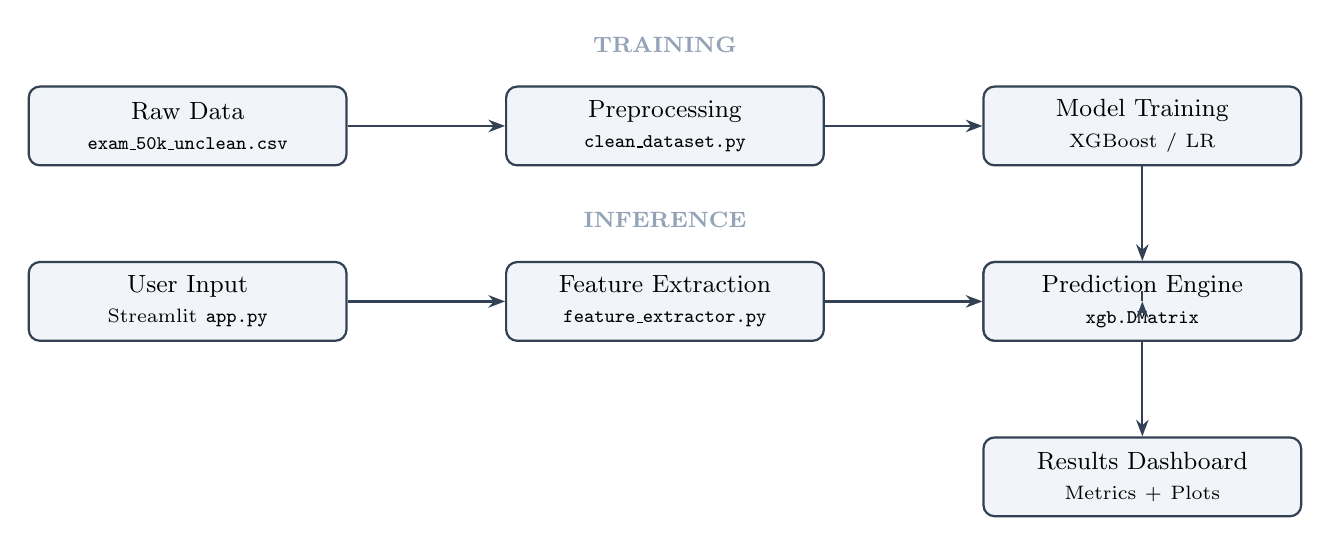
\begin{tikzpicture}[
    node distance=1.2cm and 2cm,
    every node/.style={font=\small},
    block/.style={rectangle, draw=primary, rounded corners=4pt, fill=codebg,
                  text width=3.8cm, minimum height=1cm, align=center,
                  line width=0.8pt},
    arrow/.style={-{Stealth[length=6pt]}, line width=0.8pt, color=primary}
]

% Training Pipeline
\node[block] (data) {Raw Data\\{\scriptsize\texttt{exam\_50k\_unclean.csv}}};
\node[block, right=of data] (clean) {Preprocessing\\{\scriptsize\texttt{clean\_dataset.py}}};
\node[block, right=of clean] (train) {Model Training\\{\scriptsize XGBoost / LR}};
\node[block, below=of train] (save) {Serialisation\\{\scriptsize\texttt{.json} / \texttt{.pkl}}};

% Inference Pipeline
\node[block, below=of data] (input) {User Input\\{\scriptsize Streamlit \texttt{app.py}}};
\node[block, right=of input] (feat) {Feature Extraction\\{\scriptsize\texttt{feature\_extractor.py}}};
\node[block, right=of feat] (pred) {Prediction Engine\\{\scriptsize\texttt{xgb.DMatrix}}};
\node[block, below=of pred] (out) {Results Dashboard\\{\scriptsize Metrics + Plots}};

% Arrows
\draw[arrow] (data) -- (clean);
\draw[arrow] (clean) -- (train);
\draw[arrow] (train) -- (save);
\draw[arrow] (save) -- (pred);
\draw[arrow] (input) -- (feat);
\draw[arrow] (feat) -- (pred);
\draw[arrow] (pred) -- (out);

% Labels
\node[above=0.3cm of clean, color=muted, font=\footnotesize\bfseries] {TRAINING};
\node[above=0.3cm of feat, color=muted, font=\footnotesize\bfseries] {INFERENCE};

\end{tikzpicture}
\end{center}

\subsection{Repository Structure}
\begin{lstlisting}[language={}, basicstyle=\ttfamily\footnotesize, frame=none, backgroundcolor=\color{codebg}]
genai-project/
  app.py                    # Streamlit web application
  feature_extractor.py      # 25-feature extraction module
  requirements.txt          # Python dependencies
  model/
    xg_model.pkl            # LabelEncoder pipeline
  files/
    xgb_reg_model_A.json    # XGBoost Regressor (text-only)
    xgb_clf_model_A.json    # XGBoost Classifier (text-only)
  notebooks/
    comparer/               # Model comparison notebook
    all_features_xgboost/   # All-features XGBoost notebook
    linear_regression_text/ # Linear Regression notebook
  raw_dataset/
    exam_dataset_50k_unclean.csv
  cleaned_dataset/
    exam_dataset_50k_cleaned.csv
\end{lstlisting}

% ============================================================================
%  8. APPLICATION
% ============================================================================
\section{Application Interface}\label{sec:app}

The production application (\texttt{app.py}) is built with \textbf{Streamlit} and provides two pages:

\subsection{Analysis Tool}
\begin{enumerate}[leftmargin=2em]
    \item The user inputs question text, four answer options, subject tier ($1$–$5$), misconception count, and construct frequency.
    \item \texttt{feature\_extractor.py} computes all 25 features.
    \item An \texttt{xgb.DMatrix} is constructed and fed through both the regressor and classifier boosters.
    \item A \textbf{heuristic bias adjustment} nudges the classifier's softmax probabilities based on the user-provided subject tier:
    \begin{itemize}
        \item Tiers 1–2 $\rightarrow$ slight Easy weight
        \item Tier 3 $\rightarrow$ slight Medium weight
        \item Tiers 4–5 $\rightarrow$ increased Hard weight
    \end{itemize}
    \item Results are displayed as: predicted class, difficulty $p$-value, model confidence, class-probability bar chart, and a feature-detail table.
\end{enumerate}

\subsection{About the Model}
A documentation page describing the architecture, feature extraction methodology, performance metrics, and known limitations.

\subsection{Design}
The interface follows a \textbf{dark-mode, slate-palette} design with custom CSS:
\begin{itemize}[leftmargin=2em]
    \item Background: \texttt{\#0f172a} (Slate-900)
    \item Metric cards with \texttt{\#1e293b} borders
    \item Inter typeface for readability
    \item Monospace feature values (\texttt{JetBrains Mono})
\end{itemize}

% ============================================================================
%  9. HEURISTIC ADJUSTMENT
% ============================================================================
\section{Post-Prediction Heuristic Adjustment}\label{sec:heuristic}

Because the text-only model has limited contextual awareness, a \textbf{lightweight heuristic layer} adjusts classifier probabilities after inference:

\begin{equation}
    P'(c) = \frac{P(c) \cdot w_c}{\sum_{j} P(j) \cdot w_j}
\end{equation}

\noindent Where $w_c$ are tier-dependent weight multipliers:

\begin{center}
\renewcommand{\arraystretch}{1.2}
\begin{tabular}{l ccc}
    \toprule
    \textbf{Condition} & $w_{\text{Easy}}$ & $w_{\text{Medium}}$ & $w_{\text{Hard}}$ \\
    \midrule
    Short \& simple ($W < 4$, complexity $< 2$) & 5.0 & 1.0 & 1.0 \\
    Tier $\leq 2$, complexity $< 6$             & 1.5 & 1.0 & 1.0 \\
    Tier $= 3$, complexity $< 6$                & 1.0 & 1.3 & 1.0 \\
    Tier $= 4$, complexity $< 6$                & 1.0 & 1.2 & 1.5 \\
    Tier $= 5$, complexity $< 6$                & 1.0 & 1.0 & 4.0 \\
    Otherwise (complex text)                     & 1.0 & 1.0 & 1.0 \\
    \bottomrule
\end{tabular}
\end{center}

\noindent This ensures subject-tier metadata is incorporated without overriding strong textual signals.

% ============================================================================
%  10. LIMITATIONS
% ============================================================================
\section{Limitations \& Known Issues}\label{sec:limitations}

\begin{enumerate}[leftmargin=2em]
    \item \textbf{Text-Only Analysis:} The model cannot parse images, diagrams, or graphs. Geometry questions reliant on visual context may be misclassified.

    \item \textbf{Class Imbalance:} The severe Easy-class dominance ($\sim$80\%) causes the classifier to under-predict Hard and Medium classes. Mitigation strategies (SMOTE, class weights) have not yet been applied.

    \item \textbf{Multicollinearity:} Features like \texttt{text\_length} and \texttt{word\_count} are highly correlated, potentially distorting feature-importance interpretation. SHAP analysis is recommended.

    \item \textbf{Synthetic Data Bias:} The training dataset contains synthetic variations. Real-world questions with unusual formatting may yield lower-confidence predictions.

    \item \textbf{Language Support:} Feature extraction is optimised for English-language mathematics. Non-English text will produce inaccurate features.

    \item \textbf{Potential Target Leakage:} The \texttt{subject\_difficulty\_tier} feature should be verified to ensure it is not derived from the target variable itself.
\end{enumerate}

% ============================================================================
%  11. FUTURE WORK
% ============================================================================
\section{Future Work}\label{sec:future}

\subsection{Short-Term Improvements}
\begin{itemize}[leftmargin=2em]
    \item Apply \textbf{class-weight balancing} or \textbf{SMOTE} to address the imbalance problem.
    \item Use \textbf{SHAP values} for feature-importance interpretation instead of raw XGBoost importances.
    \item Implement \textbf{hyperparameter tuning} via Bayesian optimisation (Optuna/Hyperopt).
    \item Drop highly correlated features to reduce multicollinearity.
\end{itemize}

\subsection{Milestone 2 — Agentic AI Framework}
\begin{itemize}[leftmargin=2em]
    \item \textbf{LLM Reasoning:} Use large language models (Gemini / GPT) to solve questions step-by-step and measure \emph{conceptual} complexity rather than lexical proxies.
    \item \textbf{RAG for Curriculum Alignment:} Retrieval-Augmented Generation to compare questions against educational standards.
    \item \textbf{Multi-Modal Processing:} Vision-Language Models for diagram- and graph-dependent questions.
    \item \textbf{Iterative Feedback Loops:} Agentic workflows simulating student failure modes to refine difficulty estimates.
\end{itemize}

% ============================================================================
%  12. CONCLUSION
% ============================================================================
\section{Conclusion}\label{sec:conclusion}

This project demonstrates that a combination of lightweight NLP feature engineering and gradient-boosted tree models can provide a meaningful automated estimate of examination question difficulty. The text-only XGBoost model achieves an $R^2$ of $\sim$0.57 and $\sim$83\% classification accuracy, while the all-features variant reaches $R^2 = 0.976$ when post-administration data is available.

The Streamlit application provides an accessible interface for educators to obtain instant difficulty assessments, and the modular architecture (separate feature extractor, serialised models, heuristic layer) enables straightforward future extension.

Key next steps include addressing classimbalance, integrating SHAP-based interpretability, and evolving toward an agentic LLM-based framework for deeper conceptual difficulty analysis.

% ============================================================================
%  APPENDIX
% ============================================================================
\appendix
\section{Technology Stack}\label{app:tech}

\begin{center}
\renewcommand{\arraystretch}{1.3}
\begin{tabular}{ll}
    \toprule
    \textbf{Component} & \textbf{Technology} \\
    \midrule
    Language        & Python 3.10+ \\
    ML Framework    & XGBoost $\geq$ 2.0, scikit-learn $\geq$ 1.3 \\
    Data Processing & Pandas $\geq$ 2.0, NumPy $\geq$ 1.24 \\
    Visualisation   & Matplotlib $\geq$ 3.7, Seaborn $\geq$ 0.12 \\
    Web Framework   & Streamlit $\geq$ 1.30 \\
    Serialisation   & Joblib $\geq$ 1.3, XGBoost JSON \\
    \bottomrule
\end{tabular}
\end{center}

\section{Feature Vector Specification}\label{app:features}

The complete ordered feature vector $\mathbf{x} \in \mathbb{R}^{25}$ used by the deployed models:

\begin{center}
\small
\renewcommand{\arraystretch}{1.15}
\begin{longtable}{c l l}
    \toprule
    \textbf{\#} & \textbf{Feature Name} & \textbf{Type} \\
    \midrule
    \endfirsthead
    \toprule
    \textbf{\#} & \textbf{Feature Name} & \textbf{Type} \\
    \midrule
    \endhead
    1  & \texttt{text\_length}              & Integer \\
    2  & \texttt{word\_count}               & Integer \\
    3  & \texttt{sentence\_count}           & Integer \\
    4  & \texttt{avg\_word\_length}          & Float \\
    5  & \texttt{latex\_command\_count}      & Integer \\
    6  & \texttt{has\_latex}                 & Binary \\
    7  & \texttt{latex\_density}             & Float \\
    8  & \texttt{math\_operator\_count}      & Integer \\
    9  & \texttt{number\_count}              & Integer \\
    10 & \texttt{vocab\_richness}            & Float \\
    11 & \texttt{text\_complexity\_score}     & Float \\
    12 & \texttt{answer\_a\_length}           & Integer \\
    13 & \texttt{answer\_b\_length}           & Integer \\
    14 & \texttt{answer\_c\_length}           & Integer \\
    15 & \texttt{answer\_d\_length}           & Integer \\
    16 & \texttt{avg\_answer\_length}         & Float \\
    17 & \texttt{answer\_length\_variance}    & Float \\
    18 & \texttt{has\_advanced\_terms}        & Binary \\
    19 & \texttt{has\_algebra\_terms}         & Binary \\
    20 & \texttt{has\_geometry\_terms}        & Binary \\
    21 & \texttt{has\_stats\_terms}           & Binary \\
    22 & \texttt{num\_misconceptions}         & Integer \\
    23 & \texttt{has\_misconception}          & Binary \\
    24 & \texttt{subject\_difficulty\_tier}   & Ordinal \\
    25 & \texttt{construct\_frequency}        & Integer \\
    \bottomrule
\end{longtable}
\end{center}

\end{document}
